\documentclass[a4paper,12pt]{article}
\usepackage[russian]{babel}
\usepackage[T2A]{fontenc}
\usepackage[utf8]{inputenc}
\usepackage{geometry}
\usepackage{amsmath}
\usepackage{graphicx}
\usepackage{cancel}
\usepackage{float} 
\usepackage{xcolor}
\usepackage{array}
\usepackage{caption}
\usepackage{booktabs}
\usepackage{amssymb}
\usepackage{subcaption}
\usepackage{pgfplots}
\pgfplotsset{compat=1.18}
\usetikzlibrary{arrows.meta, matrix}
\usepackage{capt-of}
\usepackage{multirow}
\usepackage[siunitx]{circuitikz}
\usepackage[bottom]{footmisc}
\usepackage{tcolorbox}
\usepackage{nicematrix}
\usepackage{tikz}
\usetikzlibrary{positioning, arrows.meta}

% --- hyperref ОДИН РАЗ ---
\usepackage{hyperref}
\hypersetup{linktoc=page}
\hypersetup{
	colorlinks=true,
	linkcolor=red,
	citecolor=red,
	urlcolor=red,
	filecolor=red,
}

% --- Содержание ---
\usepackage{tocloft}
\usepackage{etoolbox}
\usepackage{hyperref}
\hypersetup{
	colorlinks=true,
	linkcolor=red,
	citecolor=red,
	urlcolor=red,
}

% Патчим \tableofcontents: текст строк — без ссылок и чёрный
% Это делается через замену \contentsline внутри TOC
\preto\tableofcontents{%
	\begingroup
	% Переопределяем contentsline так, чтобы текст был чёрным без ссылки,
	% а номер страницы — красной ссылкой
	\renewcommand{\contentsline}[4]{%
		\ifnum\pdfstrcmp{##1}{section}=0
		\vskip 4pt{\normalfont\color{black}##2}\nobreak\hfill
		{\normalfont\color{red}\hyperlink{##4}{##3}}\par
		\else\ifnum\pdfstrcmp{##1}{subsection}=0
		\vskip 2pt\hspace{1.5em}{\normalfont\color{black}##2}\nobreak\hfill
		{\normalfont\color{red}\hyperlink{##4}{##3}}\par
		\else
		\vskip 1pt\hspace{3em}{\normalfont\color{black}##2}\nobreak\hfill
		{\normalfont\color{red}\hyperlink{##4}{##3}}\par
		\fi\fi
	}%
}
\appto\tableofcontents{\endgroup}

\newcommand{\figwidth}{0.7\textwidth}

% tocloft — только для отступов, без переопределения шрифтов
\usepackage{tocloft}

% --- Листинги ---
\usepackage{listings}

\definecolor{codebg}{RGB}{250,250,252}
\definecolor{linenumcolor}{RGB}{150,150,170}
\definecolor{mathblue}{RGB}{30,100,200}
\definecolor{mathorange}{RGB}{200,100,20}
\definecolor{matlabblue}{RGB}{0,0,200}
\definecolor{matlabgreen}{RGB}{30,130,30}
\definecolor{matlaborange}{RGB}{200,80,0}

\lstdefinelanguage{Mathematica}{
	keywords={Plot, Eigenvalues, MatrixExp, RiccatiSolve, IdentityMatrix,
		Inverse, Transpose, Simplify, Eigensystem, StateSpaceModel,
		ControllabilityMatrix, MatrixRank, Export, FileNameJoin,
		NotebookDirectory, ConstantArray, ZeroMatrix, NDSolve,
		Evaluate, LineLegend, Placed, Directive, Opacity, Filling,
		FillingStyle, PlotStyle, PlotLegends, PlotRange, Frame,
		Axes, FrameLabel, GridLines, GridLinesStyle, AspectRatio,
		Style, FontFamily, FontSize, Thick, Dashed, Dotted,
		DotDashed, RGBColor, GrayLevel, LegendLayout, LabelStyle,
		Subscript, Table, Do, Module, Block, If, True, False, Automatic},
	sensitive=true,
	morecomment=[s]{(*}{*)},
	morestring=[b]",
}

\lstdefinestyle{mma}{
	language=Mathematica,
	basicstyle=\ttfamily\small,
	keywordstyle=\color{mathblue}\bfseries,
	commentstyle=\color{linenumcolor}\itshape,
	stringstyle=\color{mathorange},
	numberstyle=\tiny\color{linenumcolor},
	numbers=left,
	numbersep=10pt,
	backgroundcolor=\color{codebg},
	frame=single,
	frameround=tttt,
	framesep=4pt,
	rulecolor=\color{mathblue!40},
	breaklines=true,
	tabsize=4,
	showstringspaces=false,
	captionpos=b,
	xleftmargin=15pt,
	xrightmargin=5pt,
}

\lstdefinestyle{matlab}{
	language=Matlab,
	basicstyle=\ttfamily\small,
	keywordstyle=\color{matlabblue}\bfseries,
	commentstyle=\color{matlabgreen}\itshape,
	stringstyle=\color{matlaborange},
	numberstyle=\tiny\color{linenumcolor},
	numbers=left,
	numbersep=10pt,
	backgroundcolor=\color{codebg},
	frame=single,
	frameround=tttt,
	framesep=4pt,
	rulecolor=\color{matlabblue!30},
	breaklines=true,
	tabsize=4,
	showstringspaces=false,
	captionpos=b,
	xleftmargin=15pt,
	xrightmargin=5pt,
	escapeinside={\%*}{*)},
	morekeywords={cvx_begin,cvx_end,sdp,variable,minimize,maximize},
}

\lstset{style=mma}

\renewcommand{\lstlistingname}{Листинг}
\DeclareCaptionFormat{redlisting}{#1\textcolor{red}{#2}#3}
\captionsetup[lstlisting]{format=redlisting}

\geometry{left=1.5cm, right=2cm, bottom=2cm, top=2cm}
\captionsetup[figure]{name=Рисунок}
\captionsetup[table]{name=Таблица}
\captionsetup{labelsep=endash}


\begin{document}
	
	\begin{titlepage}
		\centering
		
		\vspace*{0.5cm}
		{\small
			Министерство науки и высшего образования Российской Федерации\\[2pt]
			Федеральное государственное автономное образовательное учреждение\\
			высшего образования\\[2pt]
			\textbf{«Национальный исследовательский университет ИТМО»}\\
		}
		
		\vspace{0.8cm}
		\hrule height 0.8pt
		\vspace{0.3cm}
		
		{\large Факультет систем управления и робототехники}
		
		\vspace{0.3cm}
		\hrule height 0.4pt
		\vspace{2.5cm}
		
		{\Huge\bfseries ОТЧЁТ}\\[0.4cm]
		{\LARGE\bfseries о лабораторной работе №4}\\[0.8cm]
		
		\begin{tcolorbox}[
			colback=gray!4,
			colframe=gray!10,
			boxrule=0.8pt,
			arc=4pt,
			left=12pt, right=12pt, top=8pt, bottom=8pt
			]
			\centering
			{\large По дисциплине:\\[4pt]}
			{\large\bfseries «Адаптивное и робастное управление»}\\[10pt]
			{\large Тема:\\[4pt]}
			{\large\bfseries «Робастное управление линейным многомерным объектом по состоянию»} \\[10pt]
			{\large Вариант: 8}
		\end{tcolorbox}
\vspace{3cm}


	\begin{minipage}{0.45\textwidth}
		\raggedright
		{\large\bfseries Студенты:}\\[4pt]
		\textit{М.\,А.~Шульпин}\\
		\textit{Е.\,Д.~Охрименко}
	\end{minipage}%
	\hfill
	\begin{minipage}{0.45\textwidth}
		\raggedleft
		{\large\bfseries Преподаватель:}\\[4pt]
		\textit{Университет ИТМО, доцент \hfill А.\,В.~Парамонов}
	\end{minipage}
		
		\vfill
		\vspace{0.4cm}
		{\large Санкт-Петербург, 2026}
	\end{titlepage}
	
	\newpage
	\tableofcontents
	
	
\newpage
\section{Общие сведения и исходные данные}

\subsection{Математическая модель объекта управления}
Рассматривается линейный многомерный объект в управляемой канонической форме:
\begin{equation}
	\dot{x} = Ax + bu + \delta(t) \quad y = Cx
	\label{eq:o}
\end{equation}
где $x \in \mathbb{R}^2$ --- вектор состояния, $u \in \mathbb{R}$ --- скалярное управление, $y \in \mathbb{R}$ --- выход объекта, $\delta(t) \in \mathbb{R}^2$ --- вектор внешних возмущений.

Матрицы объекта имеют вид:
\begin{equation}
	A = \begin{bmatrix} 0 & 1 \\ 2 & 2 \end{bmatrix} \qquad 
	b = \begin{bmatrix} 0 \\ 8 \end{bmatrix} \qquad 
	C = \begin{bmatrix} 1 & 0 \end{bmatrix}
\end{equation}
Собственные числа матрицы $A$ равны $\lambda_{1,2} = 1 \pm \sqrt{3}$, что указывает на неустойчивость объекта в разомкнутом состоянии.

Основное задающее воздействие имеет вид:
\begin{equation}
	g(t) = 2\,\text{sign}(\sin t) + 4
\end{equation}

\subsection{Истинный вектор параметров объекта}
Для синтеза робастного регулятора используется номинальная модель объекта, полученная в лабораторной работе №3. Истинный вектор параметров имеет вид:
\begin{equation}
	\theta = \begin{bmatrix} -281.5531 \\ -12.1097 \end{bmatrix}
	\label{eq:theta_true}
\end{equation}
Значение (\ref{eq:theta_true}) используется в качестве эталона при анализе параметрической ошибки $\tilde{\theta}(t)$ в разделе \ref{sec:4}.

\subsection{Эталонная модель}
Эталонная модель формируется как устойчивая система второго порядка с нулевым перерегулированием ($\sigma = 0\%$) и временем переходного процесса $t_p = 0{.}1$~с. Передаточная функция модели соответствует полиному Ньютона $(s+\omega_0)^2$, где $\omega_0 = 47{.}4386$~с$^{-1}$.

\begin{equation}
	\dot{x}_M = A_M x_M + b_M g \qquad y_M = C_M x_M
	\label{eq:oM}
\end{equation}

Матрицы эталонной модели:
\begin{equation}
	A_M = \begin{bmatrix} 0 & 1 \\ -2250.425 & -94.877 \end{bmatrix} \qquad 
	b_M = \begin{bmatrix} 0 \\ 2250.425 \end{bmatrix} \qquad 
	C_M = \begin{bmatrix} 1 & 0 \end{bmatrix}
\end{equation}
Собственные числа $A_M$ равны $-47.4386$ (кратность 2), что гарантирует асимптотическую устойчивость эталона. Цель управления --- обеспечение условия слежения: 
\begin{equation}
	\lim_{t\to\infty} \|x_M(t) - x(t)\| \leq \Delta
\end{equation}


Закон управления имеет вид:

\begin{equation}
	u = \hat{\theta}^T x + \kappa^{-1}g
\end{equation}
где $\hat{\theta}$ --- оценка вектора параметров. 

\subsection{Функция Ляпунова и матрица P}
Для синтеза алгоритма адаптации решено матричное уравнение Ляпунова, при $Q=I_2$:

\begin{equation}
	A_M^T P + P A_M = -I
\end{equation}
Получена положительно определенная матрица:
\begin{equation}
	P = \begin{bmatrix} 11.8860 & 0.0002 \\ 0.0002 & 0.0053 \end{bmatrix}
\end{equation}
Собственные числа матрицы $P$ равны $11.8860$ и $0.0053$, что подтверждает её положительную определенность. Эта матрица используется в законе настройки параметров для обеспечения устойчивости замкнутой системы.

\subsection{Внешние возмущения}
В отличие от ЛР №3, в данной работе рассматривается работа объекта в условиях внешних возмущений. Вектор возмущений:
\begin{equation}
	\delta(t) = \begin{bmatrix} 0.6\sin(10t) + 0.1\sin(50t) \\ 0.5\cos(12t) + 0.2\sin(30t) \end{bmatrix}
\end{equation}



 \newpage
 
 \section{Синтез робастных регуляторов}

\subsection{Модификация алгоритма адаптации и синтез робастного управления}

На основе результатов работы №3 модифицируем закон настройки параметров для обеспечения устойчивости при наличии возмущений $\delta(t)$. Базовый закон управления сохраняется:
\begin{equation}
	u = \hat{\theta}^T x + \kappa^{-1} g
\end{equation}

Рассматриваются два способа формирования оценки $\hat{\theta}$:


\begin{enumerate}
	\item Решение 1:  Интегральный закон заменяется на алгебраический, исключающий дрейф параметров:
	\begin{equation}
		\hat{\theta} = \gamma x b^T P e
	\end{equation}
	
	\item Решение 2: В динамический закон добавляется член утечки для ограничения норм оценок:
	\begin{equation}
		\dot{\hat{\theta}} = -\sigma \hat{\theta} + \gamma x b^T P e \qquad \hat{\theta}(0) = 0
	\end{equation}
	
\end{enumerate}
Здесь $P$ --- положительно определенная матрица из уравнения Ляпунова, $\gamma > 0$ --- коэффициент усиления, $\sigma > 0$ --- параметр модификации.


\subsection{Структура моделей в среде Simulink}

Построим системы \ref{eq:o} и \ref{eq:oM} на рисунке \ref{fig:o}:

\begin{figure}[H]
	\centering
	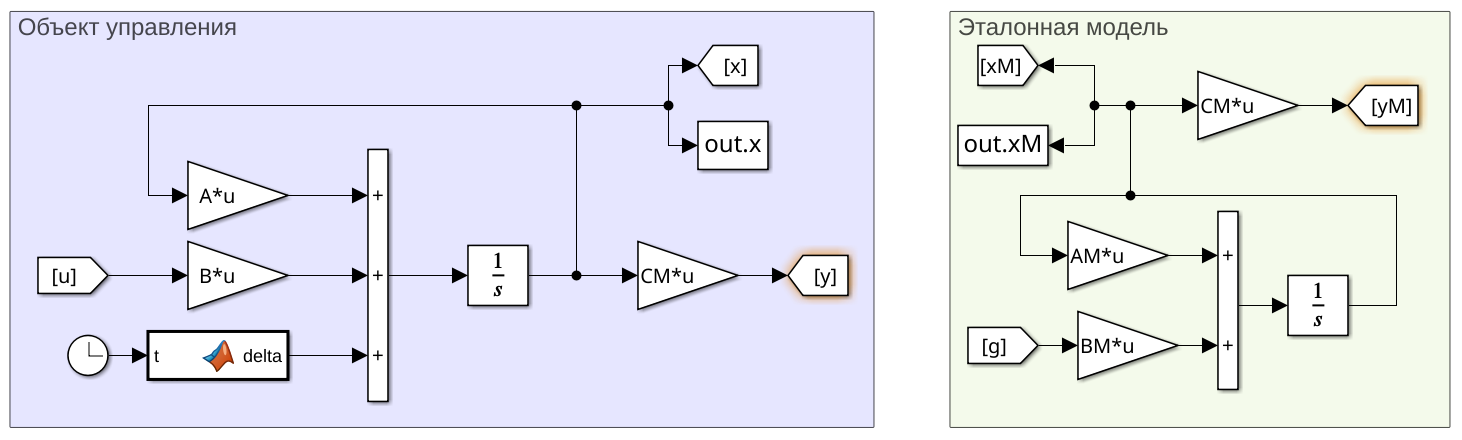
\includegraphics[width=1\textwidth]{../images/slx/objects.png}
	\caption{Схема моделирования объекта управления и эталонной модели}
	\label{fig:o}
\end{figure}

Управление приведено на рисунке \ref{fig:u}:

\begin{figure}[H]
	\centering
	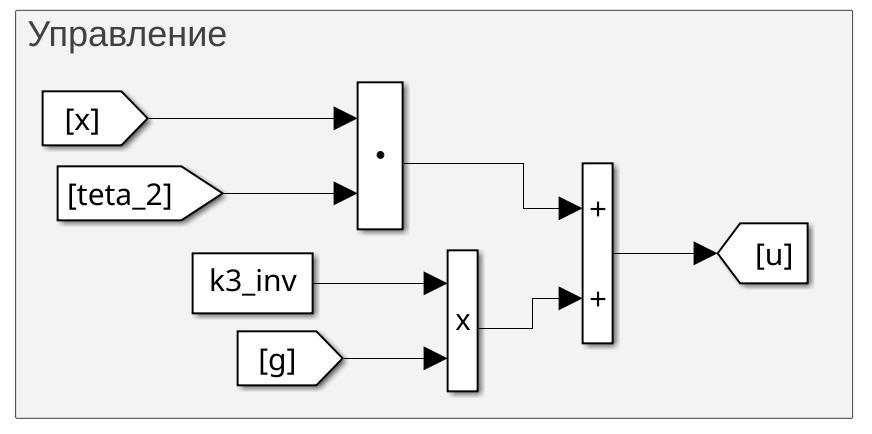
\includegraphics[width=0.5\textwidth]{../images/slx/control.png}
	\caption{Схема моделирования управления в общем виде}
	\label{fig:u}
\end{figure}

Ниже представлены оценки векторов параметра \(\theta\) (рисунки \ref{fig:t_1}--\ref{fig:t_2}):

\begin{figure}[H]
	\centering
	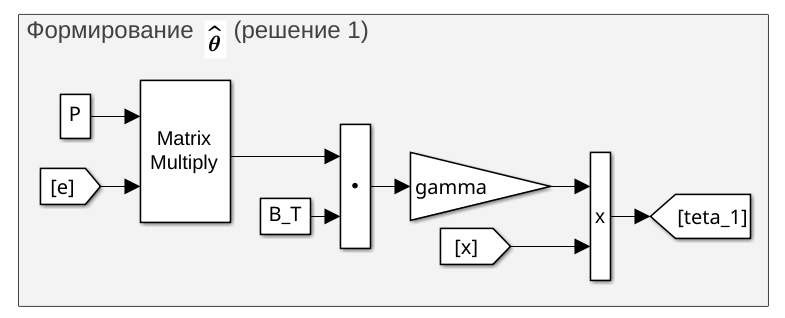
\includegraphics[width=0.6\textwidth]{../images/slx/t_1.png}
	\caption{Схема моделирования \(\hat \theta_1\)}
	\label{fig:t_1}
\end{figure}


\begin{figure}[H]
	\centering
	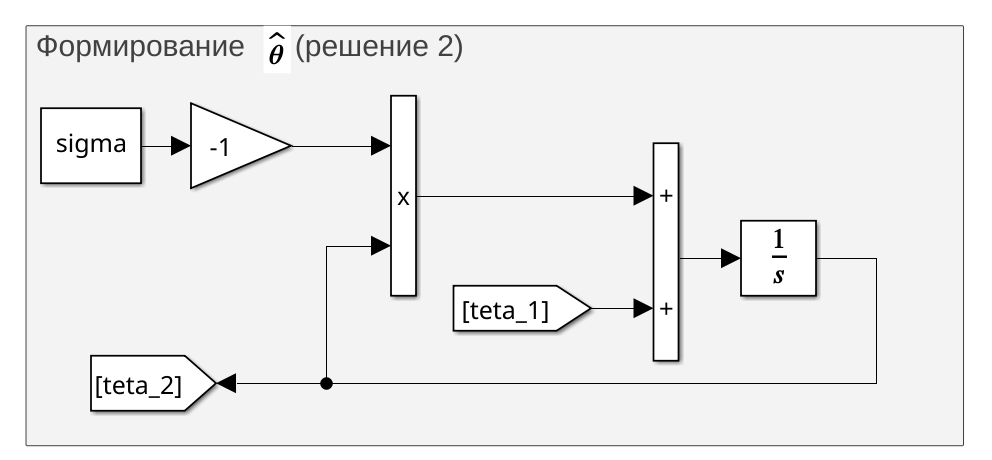
\includegraphics[width=0.6\textwidth]{../images/slx/t_2.png}
	\caption{Схема моделирования \(\hat \theta_2\)}
	\label{fig:t_2}
\end{figure}

\newpage
\section{Анализ влияния коэффициента усиления $\gamma$ на качество слежения}


Проведем моделирование системы робастного управления для трех значений коэффициента усиления: 

\begin{enumerate}
	\item $\gamma_1 = 50$;
	\item $\gamma_2 = 500$;
	\item $\gamma_3 = 5000$.
\end{enumerate}

Построим траектории $x(t)$, $x_M(t)$ и ошибку слежения $e(t)$.



\subsection{Режим работы без внешних возмущений ($\delta(t) = 0$)}

На рисунках \ref{fig:x_delta0_50}--\ref{fig:e_delta0_5000} представлены результаты моделирования при отсутствии возмущений. Увеличение коэффициента $\gamma$ приводит к уменьшению ошибки слежения $e(t)$.

\begin{figure}[H]
	\centering
	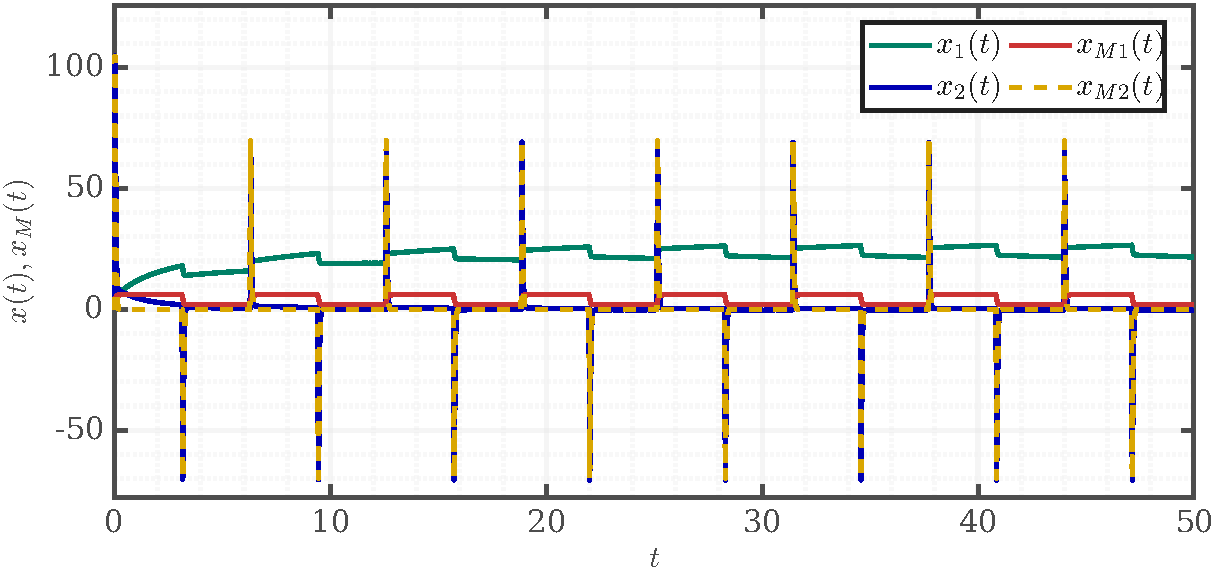
\includegraphics[width=\figwidth]{../images/task1/x_delta0_50.pdf}
	\caption{Траектории $x(t)$ и $x_M(t)$ при $\delta(t)=0$, $\gamma=50$}
	\label{fig:x_delta0_50}
\end{figure}

\begin{figure}[H]
	\centering
	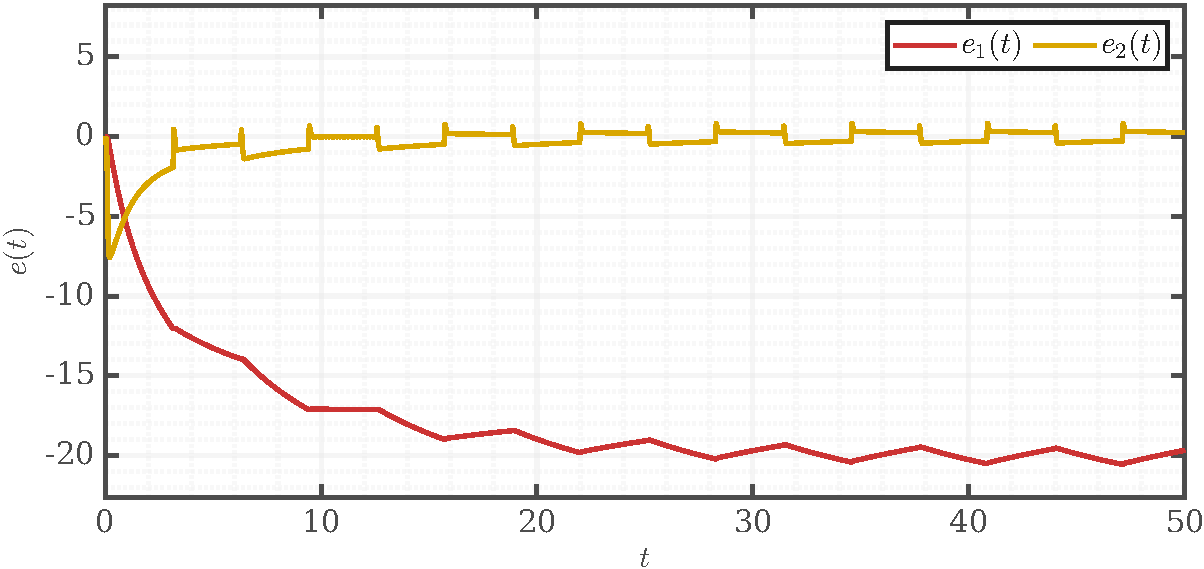
\includegraphics[width=\figwidth]{../images/task1/e_delta0_50.pdf}
	\caption{Ошибка слежения $e(t)$ при $\delta(t)=0$, $\gamma=50$}
	\label{fig:e_delta0_50}
\end{figure}

\begin{figure}[H]
	\centering
	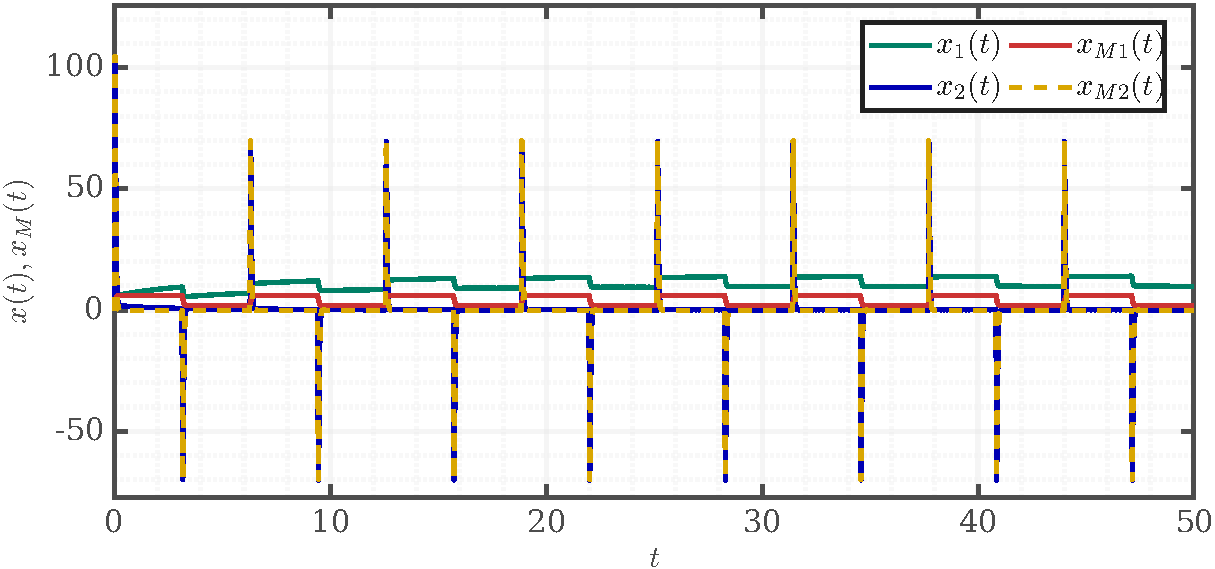
\includegraphics[width=\figwidth]{../images/task1/x_delta0_500.pdf}
	\caption{Траектории $x(t)$ и $x_M(t)$ при $\delta(t)=0$, $\gamma=500$}
	\label{fig:x_delta0_500}
\end{figure}

\begin{figure}[H]
	\centering
	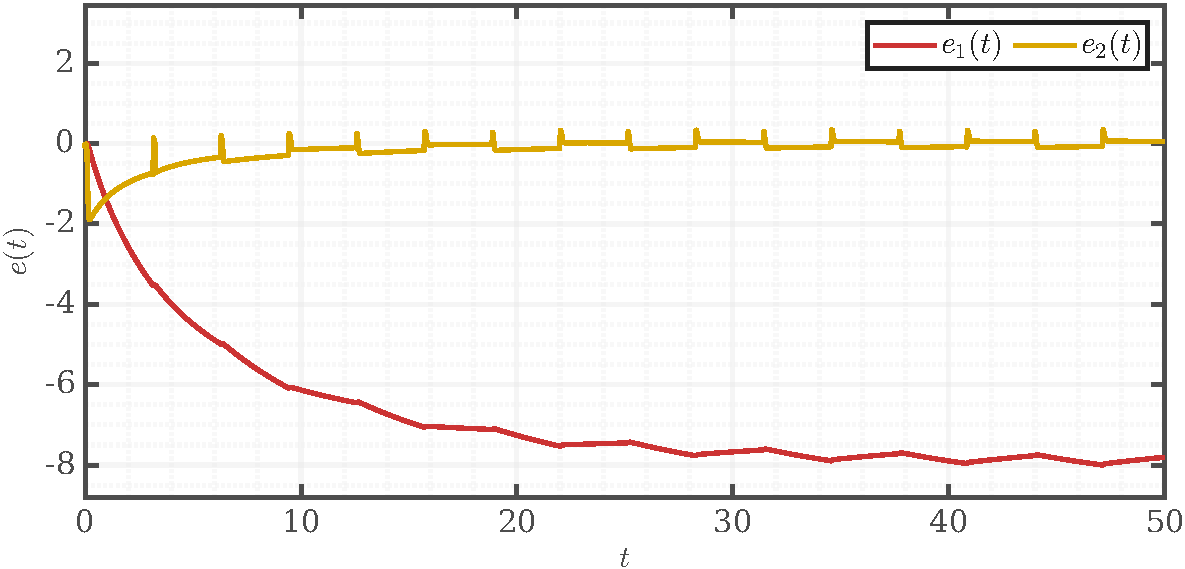
\includegraphics[width=\figwidth]{../images/task1/e_delta0_500.pdf}
	\caption{Ошибка слежения $e(t)$ при $\delta(t)=0$, $\gamma=500$}
	\label{fig:e_delta0_500}
\end{figure}

\begin{figure}[H]
	\centering
	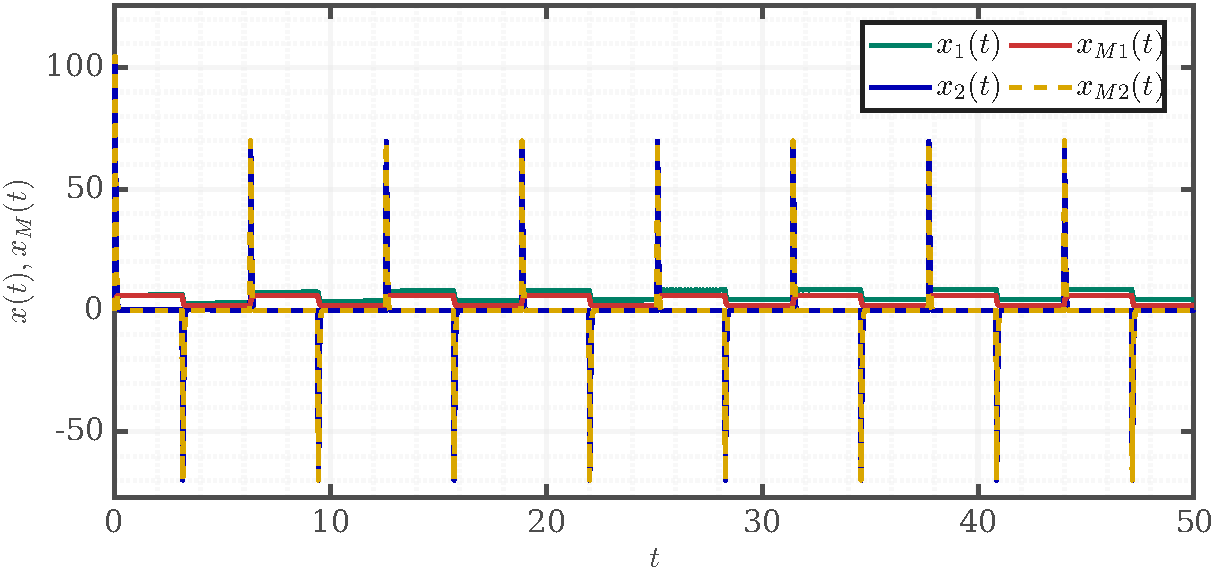
\includegraphics[width=\figwidth]{../images/task1/x_delta0_5000.pdf}
	\caption{Траектории $x(t)$ и $x_M(t)$ при $\delta(t)=0$, $\gamma=5000$}
	\label{fig:x_delta0_5000}
\end{figure}

\begin{figure}[H]
	\centering
	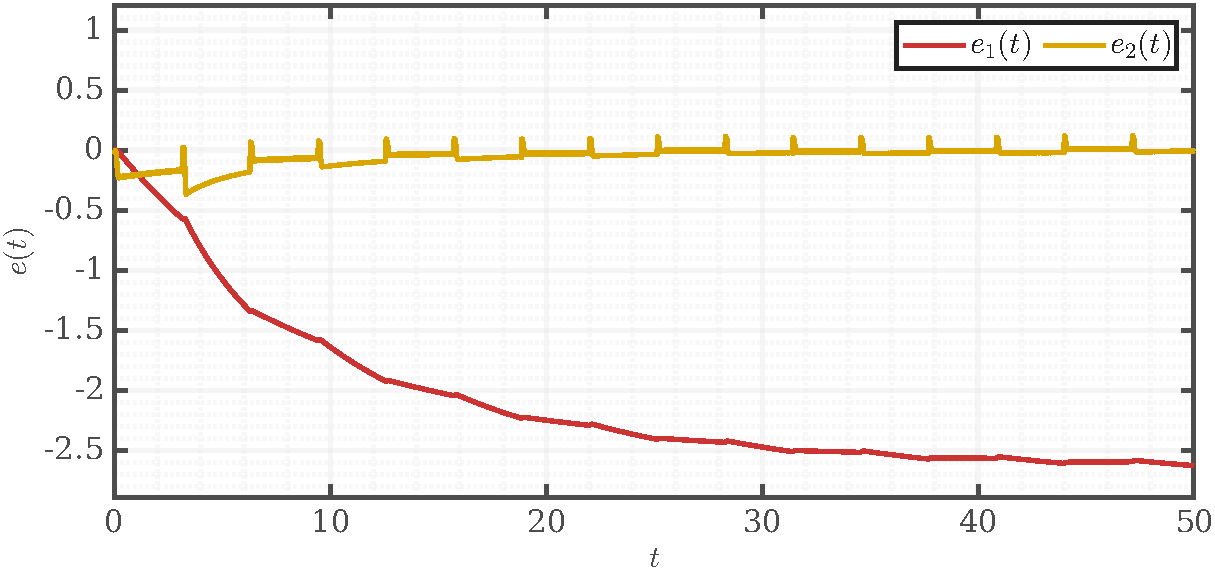
\includegraphics[width=\figwidth]{../images/task1/e_delta0_5000.pdf}
	\caption{Ошибка слежения $e(t)$ при $\delta(t)=0$, $\gamma=5000$}
	\label{fig:e_delta0_5000}
\end{figure}


\subsection{Режим работы при наличии внешних возмущений ($\delta(t) \neq 0$)}

Результаты с возмущением $\delta(t)$ приведены на рисунках \ref{fig:x_delta1_50}--\ref{fig:e_delta1_5000}. Наличие возмущения формирует установившуюся ошибку, амплитуда которой уменьшается с ростом $\gamma$.

\begin{figure}[H]
	\centering
	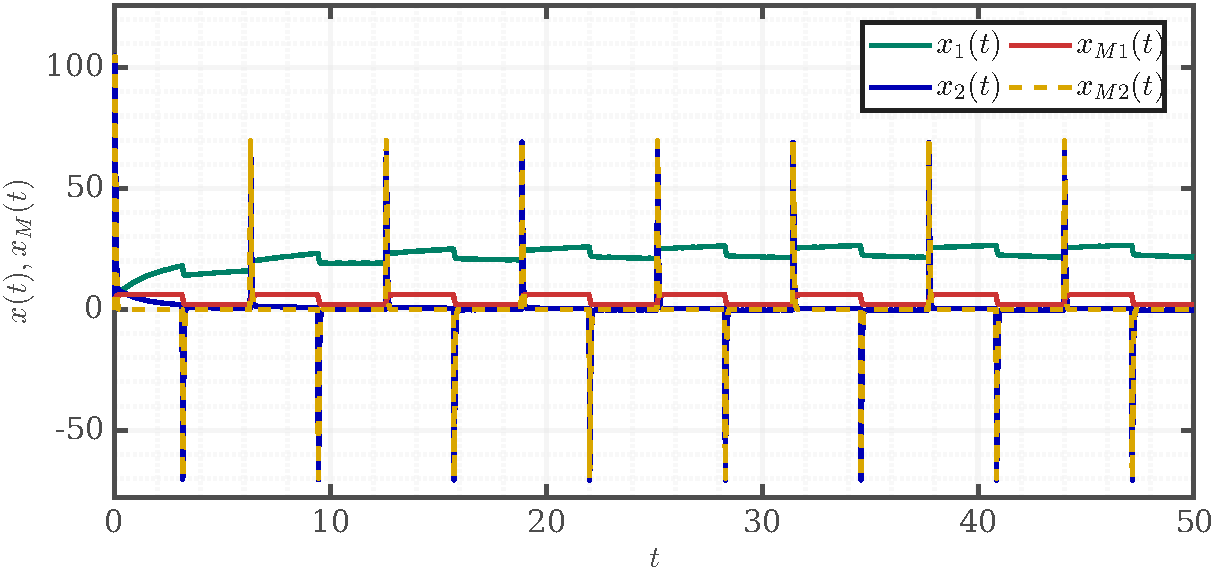
\includegraphics[width=\figwidth]{../images/task1/x_delta1_50.pdf}
	\caption{Траектории $x(t)$ и $x_M(t)$ при наличии возмущений, $\gamma=50$}
	\label{fig:x_delta1_50}
\end{figure}

\begin{figure}[H]
	\centering
	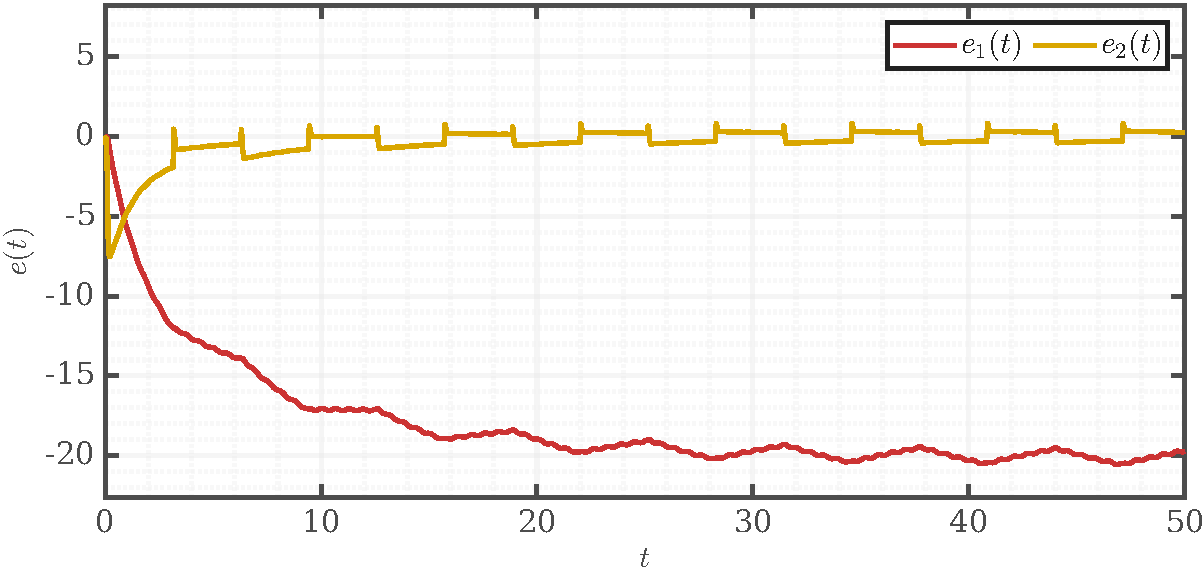
\includegraphics[width=\figwidth]{../images/task1/e_delta1_50.pdf}
	\caption{Ошибка слежения $e(t)$ при наличии возмущений, $\gamma=50$}
	\label{fig:e_delta1_50}
\end{figure}

\begin{figure}[H]
	\centering
	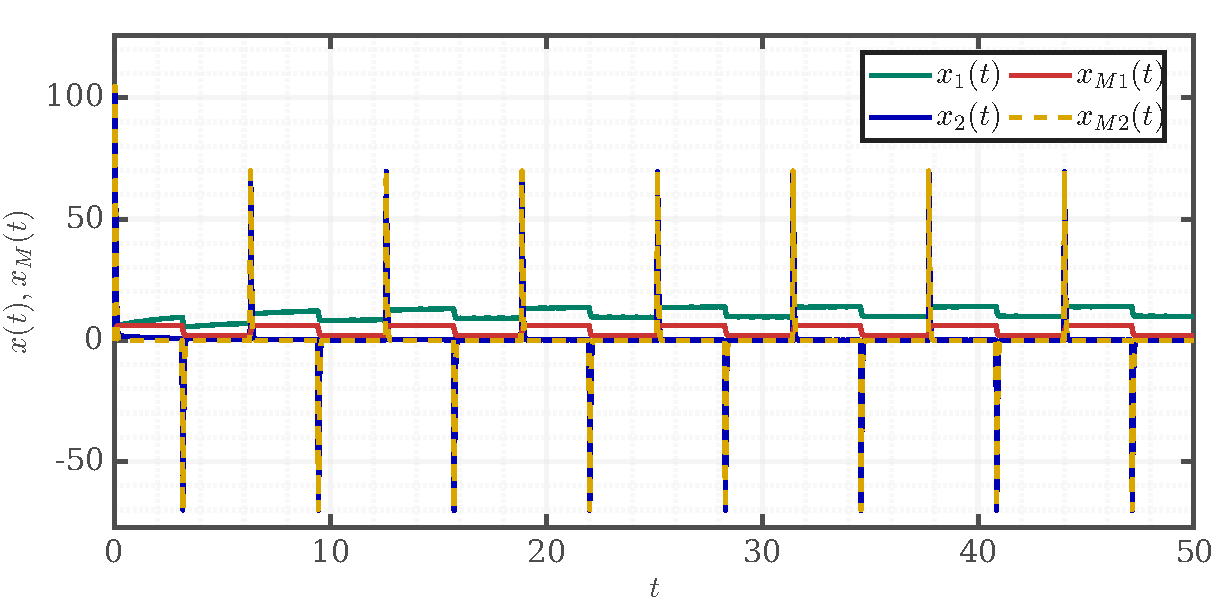
\includegraphics[width=\figwidth]{../images/task1/x_delta1_500.pdf}
	\caption{Траектории $x(t)$ и $x_M(t)$ при наличии возмущений, $\gamma=500$}
	\label{fig:x_delta1_500}
\end{figure}

\begin{figure}[H]
	\centering
	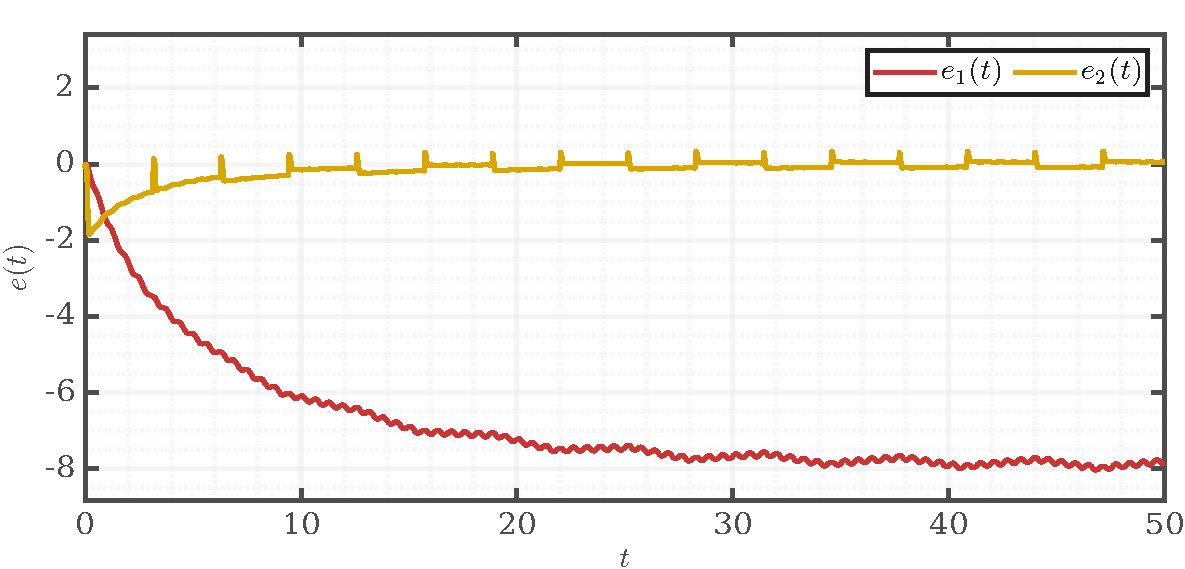
\includegraphics[width=\figwidth]{../images/task1/e_delta1_500.pdf}
	\caption{Ошибка слежения $e(t)$ при наличии возмущений, $\gamma=500$}
	\label{fig:e_delta1_500}
\end{figure}

\begin{figure}[H]
	\centering
	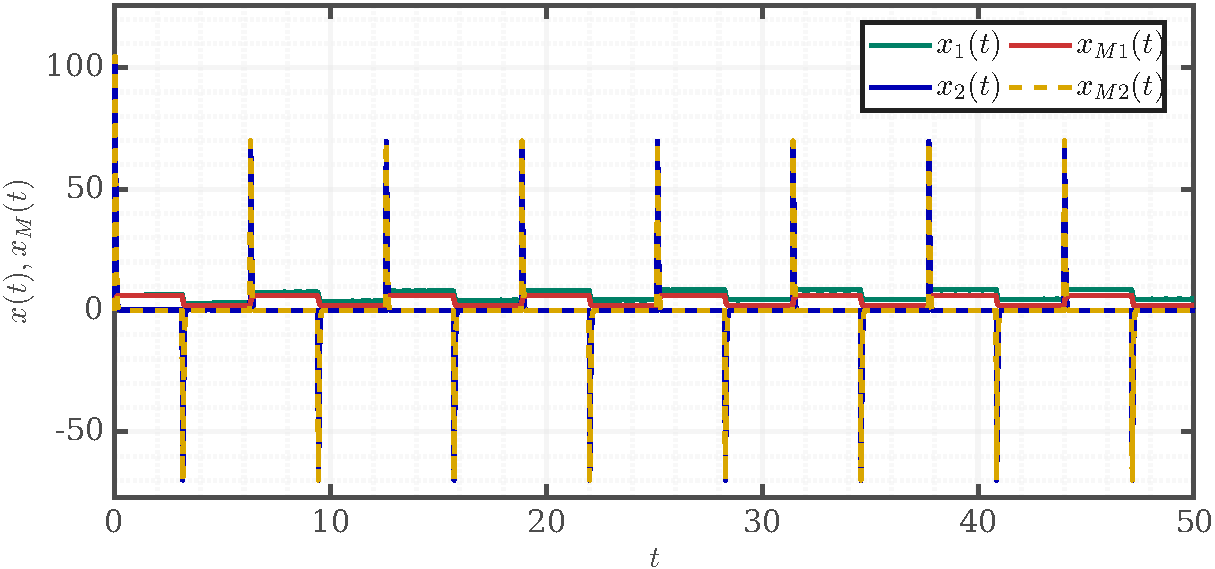
\includegraphics[width=\figwidth]{../images/task1/x_delta1_5000.pdf}
	\caption{Траектории $x(t)$ и $x_M(t)$ при наличии возмущений, $\gamma=5000$}
	\label{fig:x_delta1_5000}
\end{figure}

\begin{figure}[H]
	\centering
	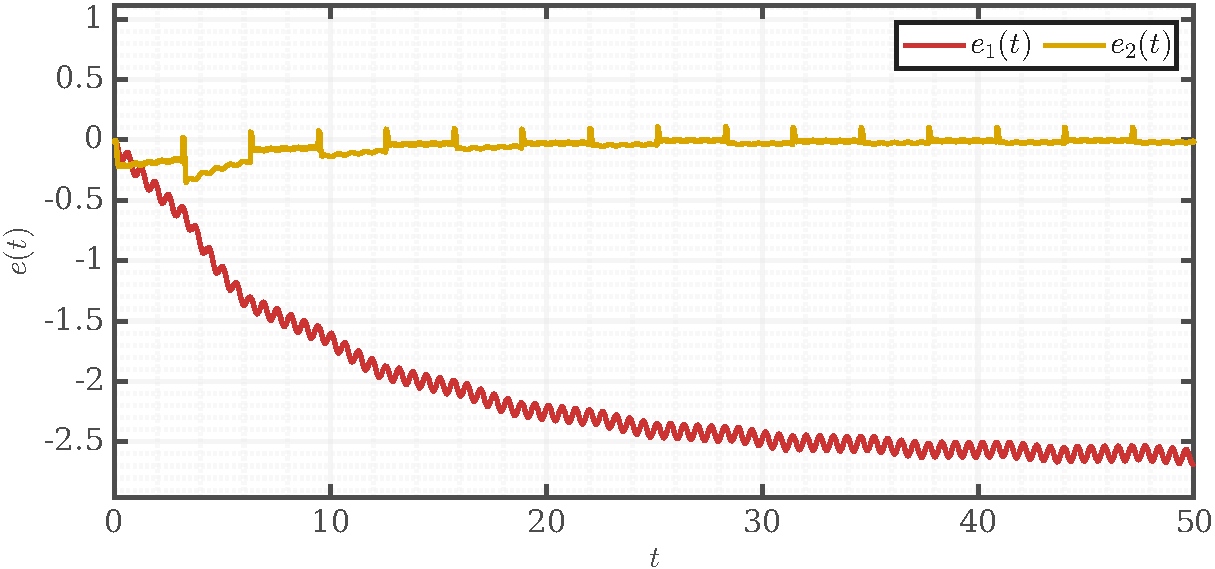
\includegraphics[width=\figwidth]{../images/task1/e_delta1_5000.pdf}
	\caption{Ошибка слежения $e(t)$ при наличии возмущений, $\gamma=5000$}
	\label{fig:e_delta1_5000}
\end{figure}


С ростом $\gamma$ амплитуда установившейся ошибки уменьшается, однако появляются колебания малой амплитуды, ненулевым возмущением, поданным на объект управления. Это подтверждает робастность алгоритма: система сохраняет устойчивость и точность слежения даже при внешних воздействиях.



\newpage

\section{Исследование влияния параметра $\sigma$-модификации}\label{sec:4}

Параметрическая ошибка определяется как разность между истинным вектором параметров и его оценкой:
\begin{equation}
	\tilde{\theta}(t) = \hat{\theta}(t) - \theta.
	\label{eq:theta_tilde}
\end{equation}

Проведем анализ робастного алгоритма для двух значений параметра утечки: $\sigma_1 = 0.05$ и $\sigma_2 = 0.005$. 
Для базового значения $\sigma_1$ исследование проводится при $\gamma \in \{500, 5000\}$, а для уменьшенного значения $\sigma_2$ --- только при оптимальном коэффициенте усиления $\gamma = 5000$.

\subsection{Режим работы без внешних возмущений ($\delta(t) = 0$)}

На рисунках ниже представлены траектории состояний, ошибки слежения и параметрические ошибки при отсутствии возмущений.

\subsubsection{Базовое значение параметра утечки $\sigma_1 = 0.05$}

При $\sigma_1 = 0.05$ член утечки обеспечивает надежную ограниченность оценок параметров даже при высоких значениях $\gamma$.

% === ГРУППА 1: sigma=0.05, gamma=500 ===
\begin{figure}[H]
	\centering
	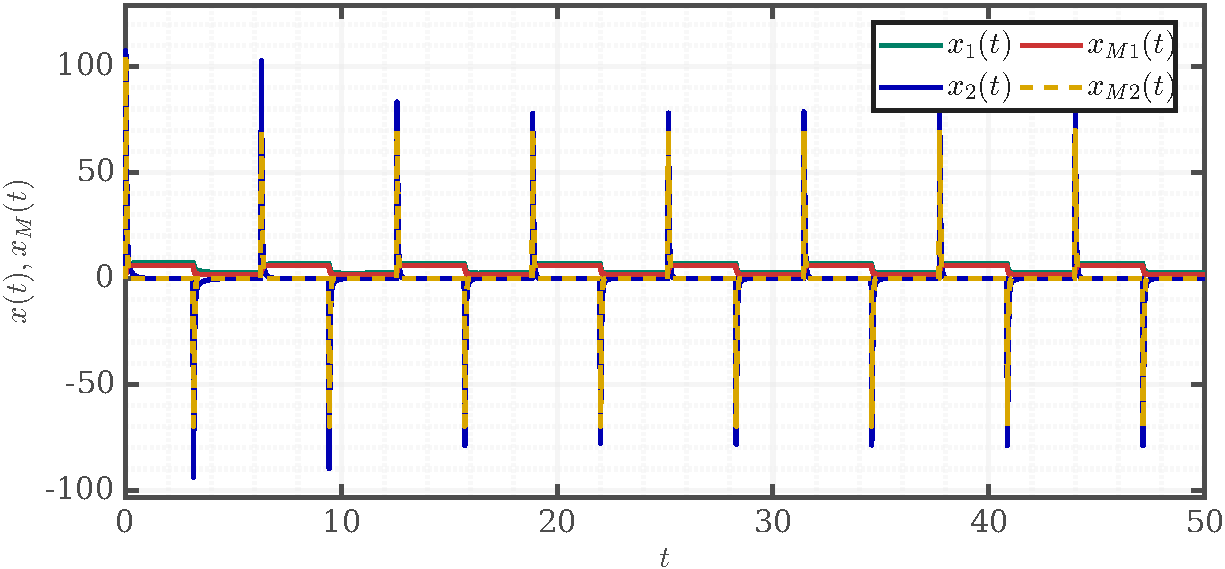
\includegraphics[width=\figwidth]{../images/task2/x_delta0_sigma0.05_gamma500.pdf}
	\caption{Траектории $x(t), x_M(t)$ при $\delta=0$, $\sigma=0.05$, $\gamma=500$}
	\label{fig:t2_x_d0_s05_g500}
\end{figure}
\begin{figure}[H]
	\centering
	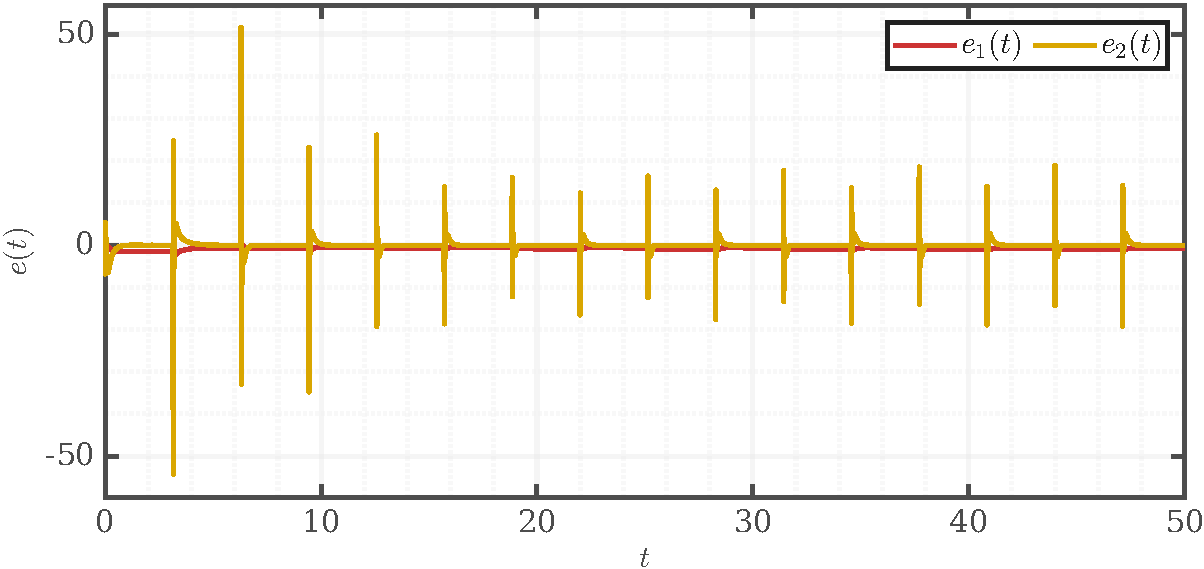
\includegraphics[width=\figwidth]{../images/task2/e_delta0_sigma0.05_gamma500.pdf}
	\caption{Ошибка $e(t)$ при $\delta=0$, $\sigma=0.05$, $\gamma=500$}
	\label{fig:t2_e_d0_s05_g500}
\end{figure}
\begin{figure}[H]
	\centering
	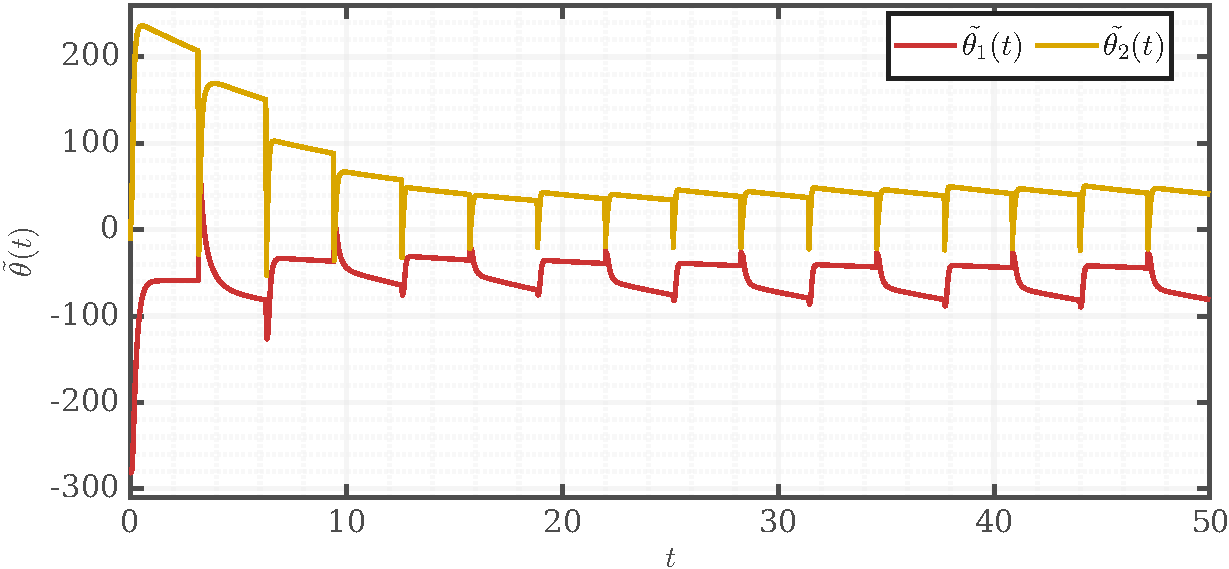
\includegraphics[width=\figwidth]{../images/task2/t_delta0_sigma0.05_gamma500.pdf}
	\caption{Параметрическая ошибка $\tilde{\theta}(t)$ при $\delta=0$, $\sigma=0.05$, $\gamma=500$}
	\label{fig:t2_t_d0_s05_g500}
\end{figure}

% === ГРУППА 2: sigma=0.05, gamma=5000 ===
\begin{figure}[H]
	\centering
	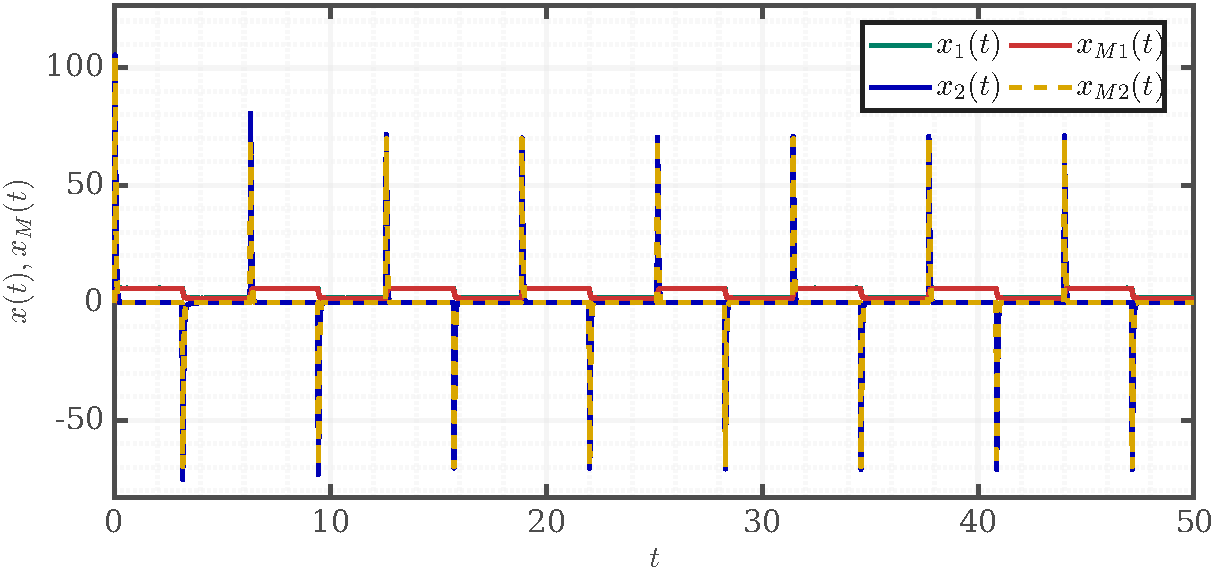
\includegraphics[width=\figwidth]{../images/task2/x_delta0_sigma0.05_gamma5000.pdf}
	\caption{Траектории $x(t), x_M(t)$ при $\delta=0$, $\sigma=0.05$, $\gamma=5000$}
	\label{fig:t2_x_d0_s05_g5k}
\end{figure}
\begin{figure}[H]
	\centering
	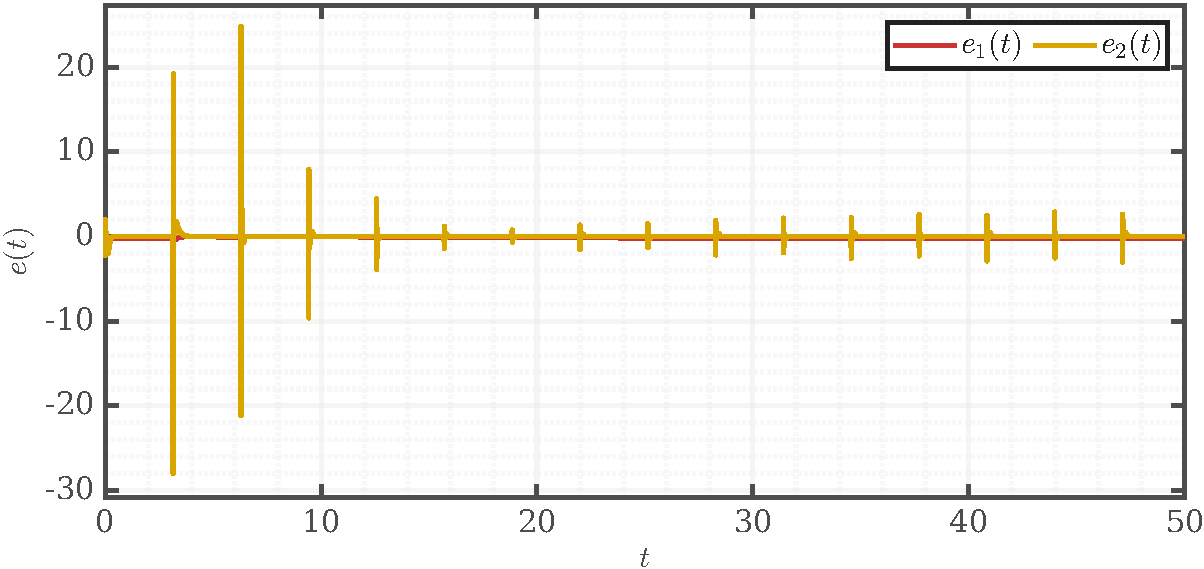
\includegraphics[width=\figwidth]{../images/task2/e_delta0_sigma0.05_gamma5000.pdf}
	\caption{Ошибка $e(t)$ при $\delta=0$, $\sigma=0.05$, $\gamma=5000$}
	\label{fig:t2_e_d0_s05_g5k}
\end{figure}
\begin{figure}[H]
	\centering
	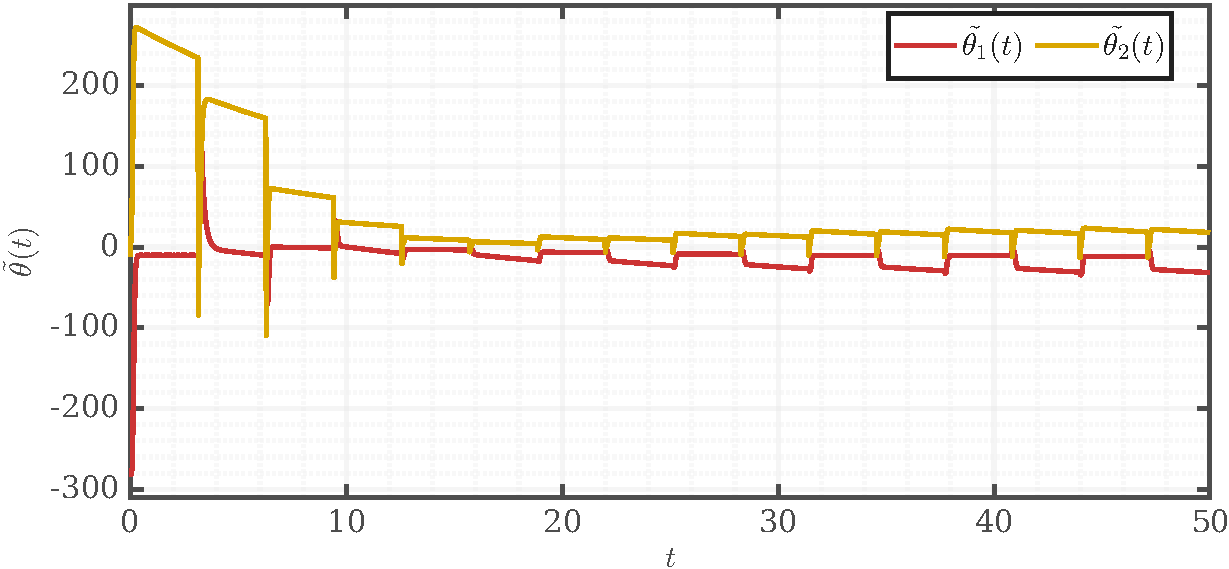
\includegraphics[width=\figwidth]{../images/task2/t_delta0_sigma0.05_gamma5000.pdf}
	\caption{Параметрическая ошибка $\tilde{\theta}(t)$ при $\delta=0$, $\sigma=0.05$, $\gamma=5000$}
	\label{fig:t2_t_d0_s05_g5k}
\end{figure}


\subsubsection{Уменьшенное значение параметра утечки $\sigma_2 = 0.005$ ($\gamma = 5000$)}

Уменьшим $\sigma$ в 10 рази проведем эксперимент только для $\gamma=5000$, так как этот коэффициент показал наилучшие результаты на предыдущем этапе.

% === ГРУППА 3: sigma=0.005, gamma=5000 (ТОЛЬКО ЭТА ПАРА!) ===
\begin{figure}[H]
	\centering
	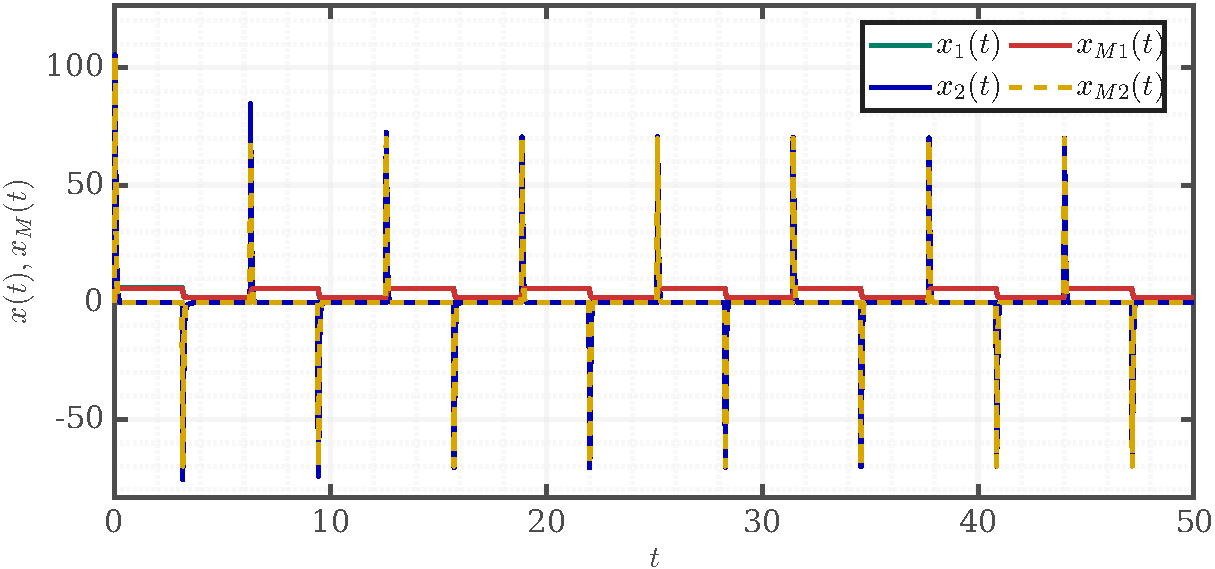
\includegraphics[width=\figwidth]{../images/task2/x_delta0_sigma0.005_gamma5000.pdf}
	\caption{Траектории $x(t), x_M(t)$ при $\delta=0$, $\sigma=0.005$, $\gamma=5000$}
	\label{fig:t2_x_d0_s005_g5k}
\end{figure}
\begin{figure}[H]
	\centering
	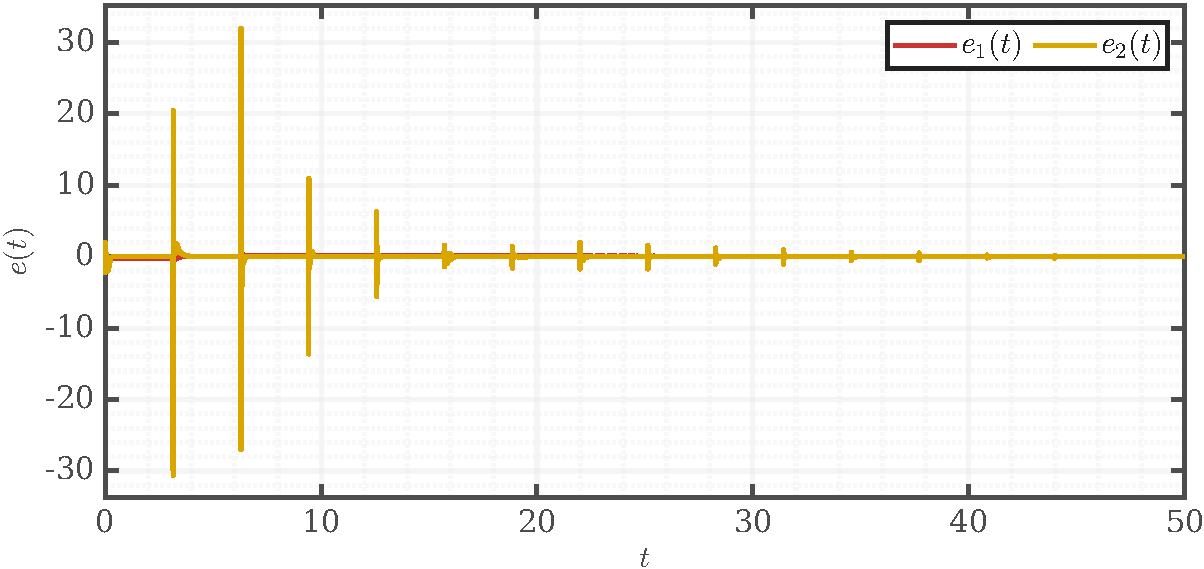
\includegraphics[width=\figwidth]{../images/task2/e_delta0_sigma0.005_gamma5000.pdf}
	\caption{Ошибка $e(t)$ при $\delta=0$, $\sigma=0.005$, $\gamma=5000$}
	\label{fig:t2_e_d0_s005_g5k}
\end{figure}
\begin{figure}[H]
	\centering
	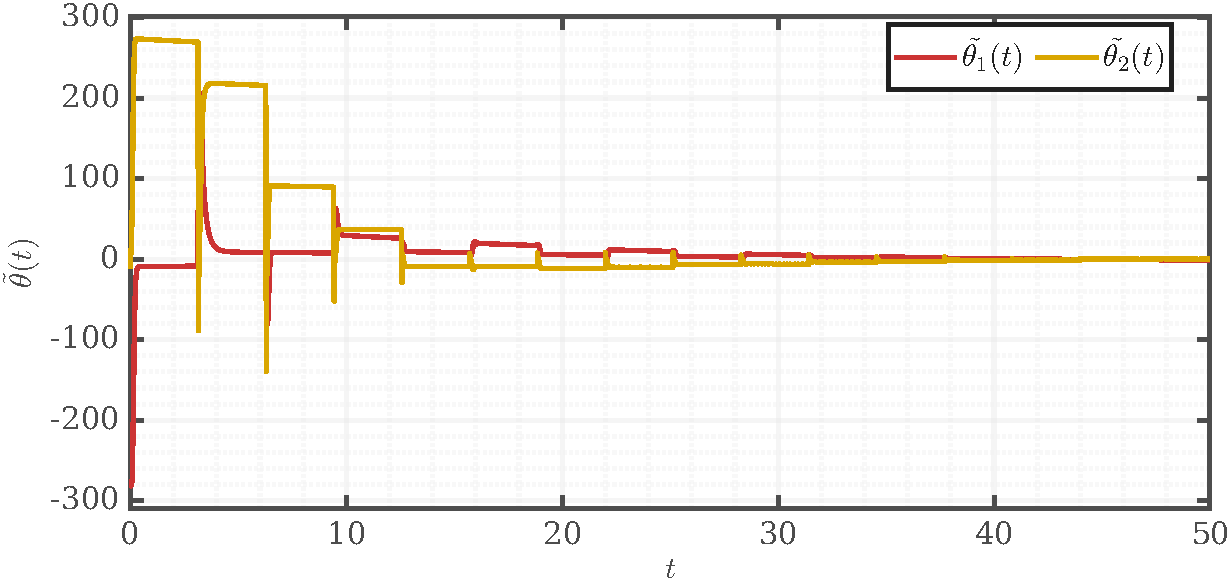
\includegraphics[width=\figwidth]{../images/task2/t_delta0_sigma0.005_gamma5000.pdf}
	\caption{Параметрическая ошибка $\tilde{\theta}(t)$ при $\delta=0$, $\sigma=0.005$, $\gamma=5000$}
	\label{fig:t2_t_d0_s005_g5k}
\end{figure}


\subsection{Режим работы при наличии внешних возмущений ($\delta(t) \neq 0$)}

Результаты с возмущением $\delta(t)$ приведены ниже. При наличии возмущений уменьшение $\sigma$ снижает установившуюся ошибку, но увеличивает чувствительность оценок $\hat{\theta}$ к высокочастотным компонентам шума.

\subsubsection{Базовое значение параметра утечки $\sigma_1 = 0.05$}

% === ГРУППА 4: sigma=0.05, gamma=500 ===
\begin{figure}[H]
	\centering
	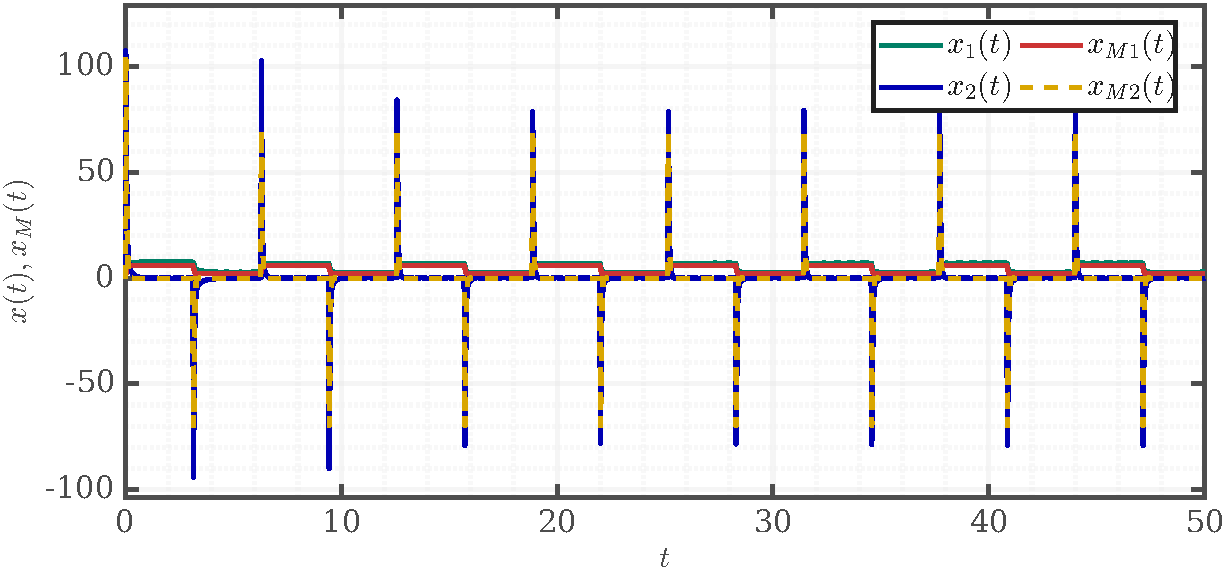
\includegraphics[width=\figwidth]{../images/task2/x_delta1_sigma0.05_gamma500.pdf}
	\caption{Траектории при $\delta \neq 0$, $\sigma=0.05$, $\gamma=500$}
	\label{fig:t2_x_d1_s05_g500}
\end{figure}
\begin{figure}[H]
	\centering
	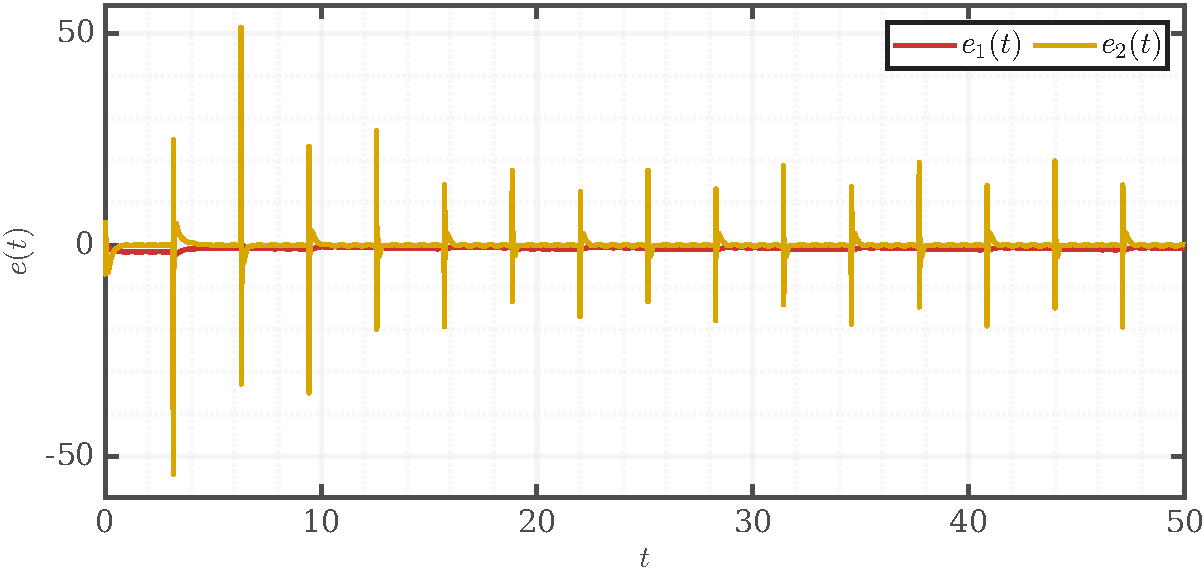
\includegraphics[width=\figwidth]{../images/task2/e_delta1_sigma0.05_gamma500.pdf}
	\caption{Ошибка $e(t)$ при $\delta \neq 0$, $\sigma=0.05$, $\gamma=500$}
	\label{fig:t2_e_d1_s05_g500}
\end{figure}
\begin{figure}[H]
	\centering
	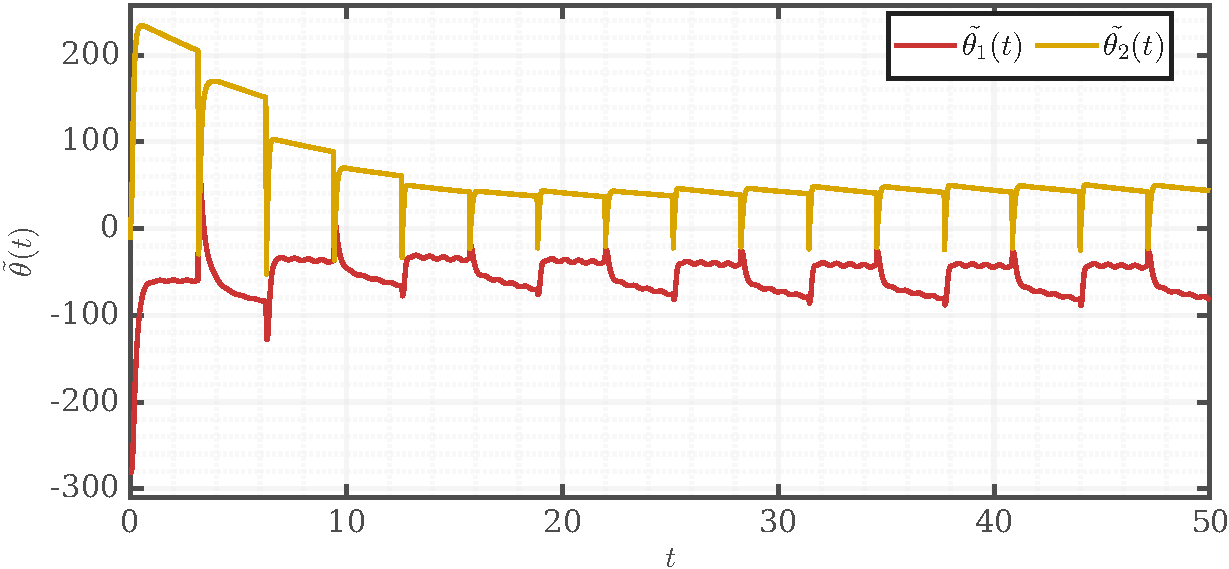
\includegraphics[width=\figwidth]{../images/task2/t_delta1_sigma0.05_gamma500.pdf}
	\caption{Параметрическая ошибка $\tilde{\theta}(t)$ при $\delta \neq 0$, $\sigma=0.05$, $\gamma=500$}
	\label{fig:t2_t_d1_s05_g500}
\end{figure}

% === ГРУППА 5: sigma=0.05, gamma=5000 ===
\begin{figure}[H]
	\centering
	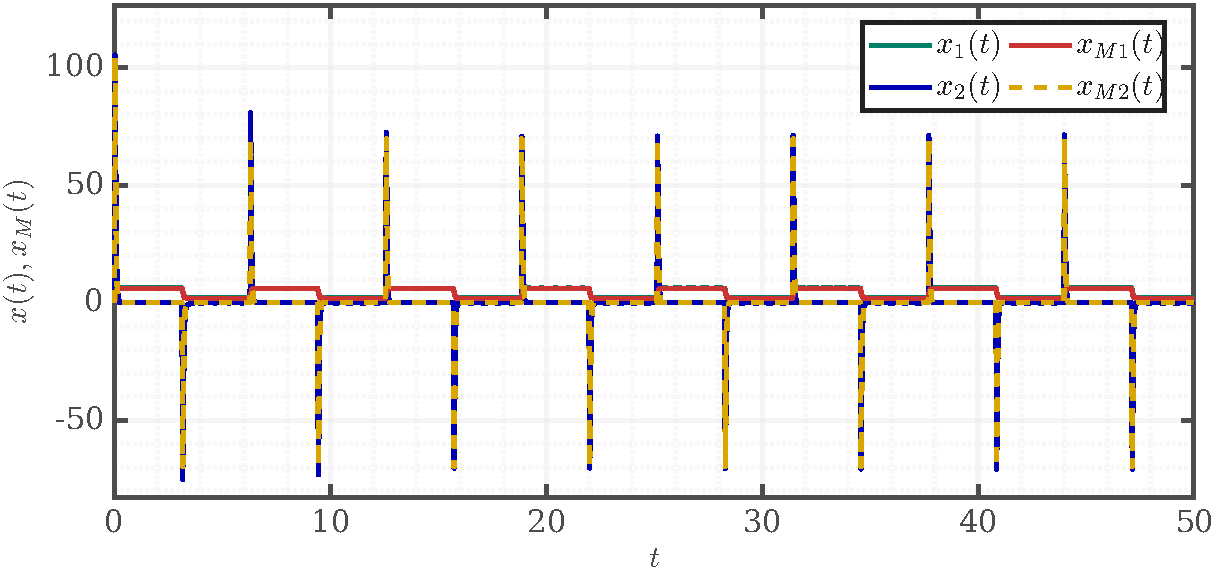
\includegraphics[width=\figwidth]{../images/task2/x_delta1_sigma0.05_gamma5000.pdf}
	\caption{Траектории при $\delta \neq 0$, $\sigma=0.05$, $\gamma=5000$}
	\label{fig:t2_x_d1_s05_g5k}
\end{figure}
\begin{figure}[H]
	\centering
	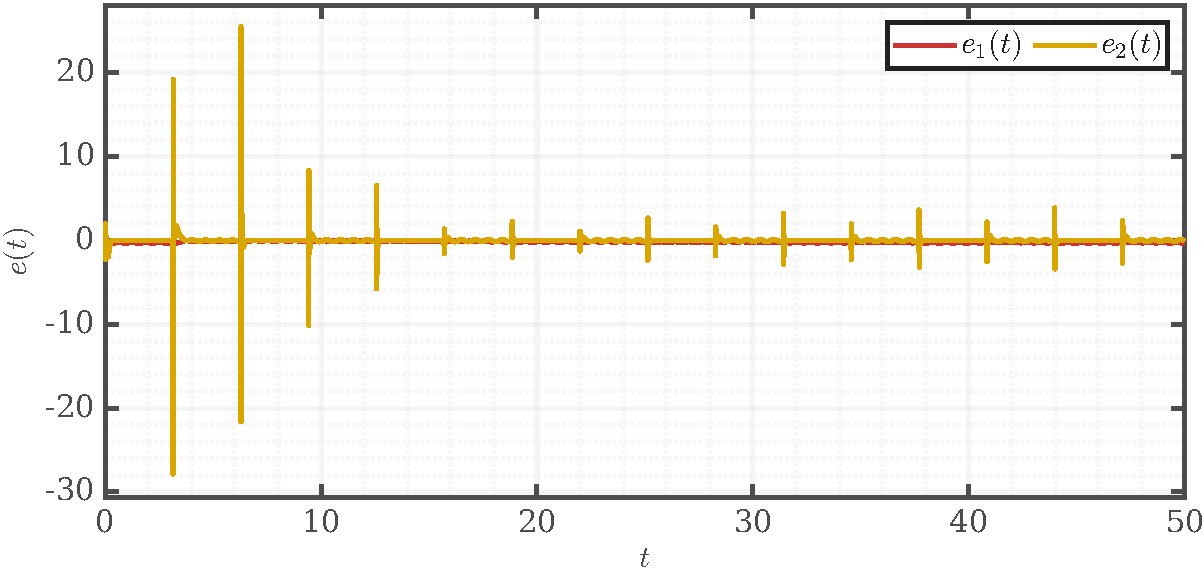
\includegraphics[width=\figwidth]{../images/task2/e_delta1_sigma0.05_gamma5000.pdf}
	\caption{Ошибка $e(t)$ при $\delta \neq 0$, $\sigma=0.05$, $\gamma=5000$}
	\label{fig:t2_e_d1_s05_g5k}
\end{figure}
\begin{figure}[H]
	\centering
	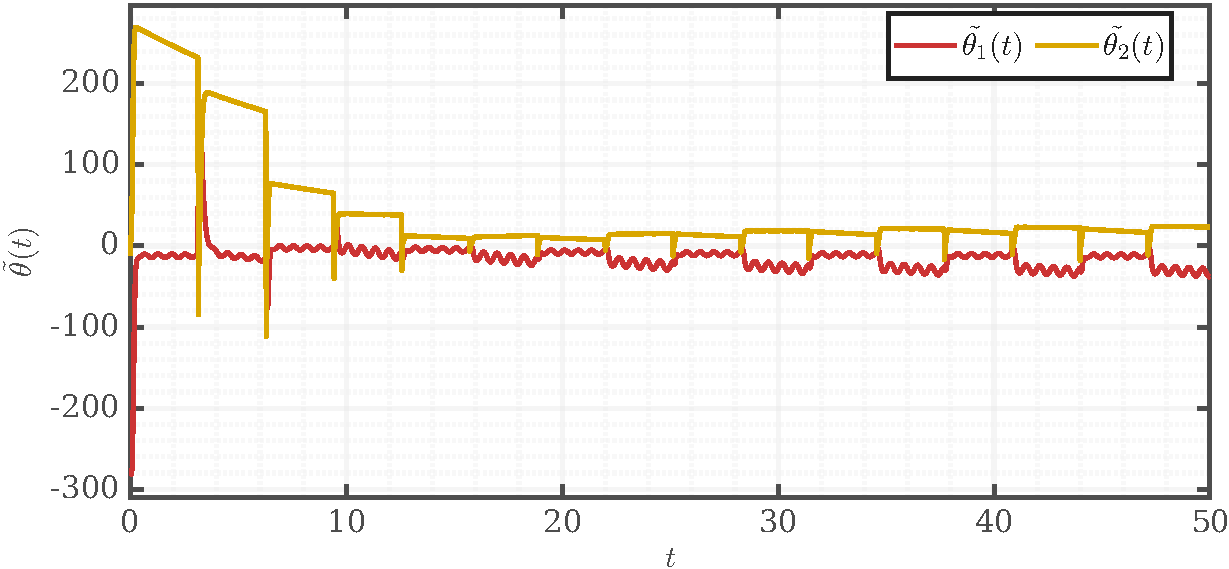
\includegraphics[width=\figwidth]{../images/task2/t_delta1_sigma0.05_gamma5000.pdf}
	\caption{Параметрическая ошибка $\tilde{\theta}(t)$ при $\delta \neq 0$, $\sigma=0.05$, $\gamma=5000$}
	\label{fig:t2_t_d1_s05_g5k}
\end{figure}


\subsubsection{Уменьшенное значение параметра утечки $\sigma_2 = 0.005$ ($\gamma = 5000$)}

% === ГРУППА 6: sigma=0.005, gamma=5000 (ТОЛЬКО ЭТА ПАРА!) ===
\begin{figure}[H]
	\centering
	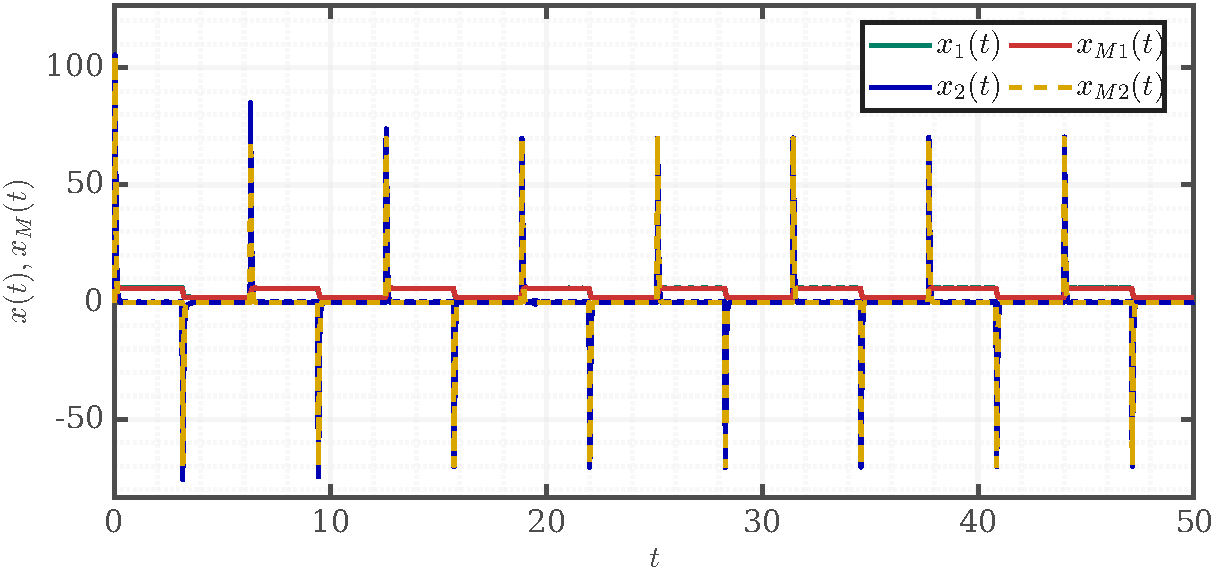
\includegraphics[width=\figwidth]{../images/task2/x_delta1_sigma0.005_gamma5000.pdf}
	\caption{Траектории при $\delta \neq 0$, $\sigma=0.005$, $\gamma=5000$}
	\label{fig:t2_x_d1_s005_g5k}
\end{figure}
\begin{figure}[H]
	\centering
	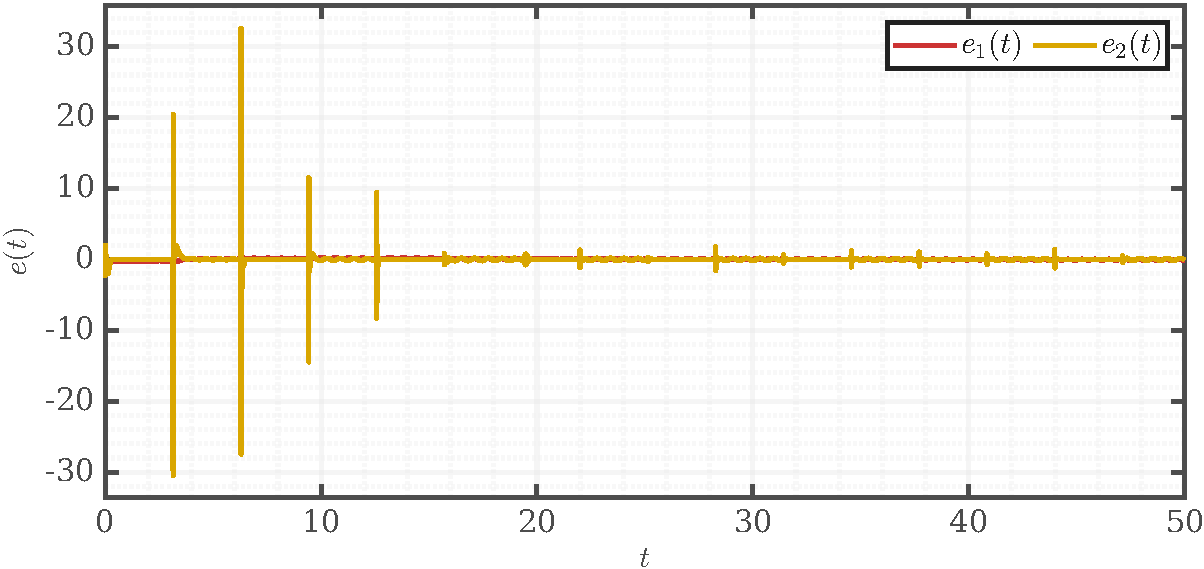
\includegraphics[width=\figwidth]{../images/task2/e_delta1_sigma0.005_gamma5000.pdf}
	\caption{Ошибка $e(t)$ при $\delta \neq 0$, $\sigma=0.005$, $\gamma=5000$}
	\label{fig:t2_e_d1_s005_g5k}
\end{figure}
\begin{figure}[H]
	\centering
	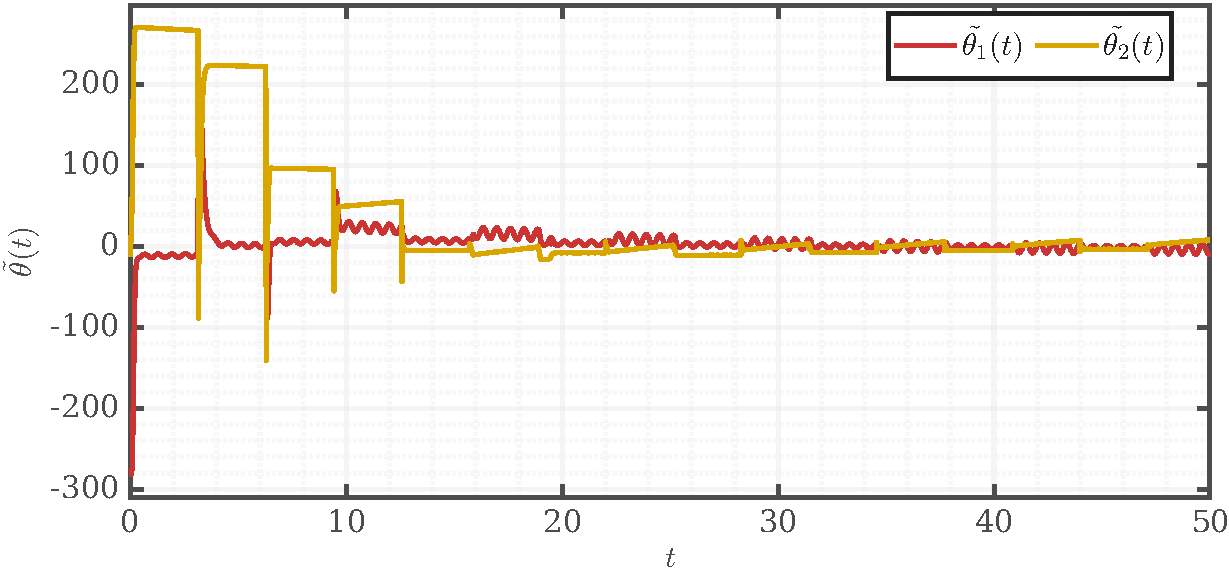
\includegraphics[width=\figwidth]{../images/task2/t_delta1_sigma0.005_gamma5000.pdf}
	\caption{Параметрическая ошибка $\tilde{\theta}(t)$ при $\delta \neq 0$, $\sigma=0.005$, $\gamma=5000$}
	\label{fig:t2_t_d1_s005_g5k}
\end{figure}


Уменьшение параметра утечки с $\sigma_1 = 0.05$ до $\sigma_2 = 0.005$ при $\gamma = 5000$ приводит к снижению установившейся ошибки слежения $e(t)$ и уменьшению смещения оценок параметров $\tilde{\theta}(t)$.

При наличии возмущений $\delta(t)$ снижение $\sigma$ улучшает точность слежения, но увеличивает чувствительность оценок $\hat{\theta}$ к высокочастотным компонентам шума. Система сохраняет устойчивость во всех режимах.


\newpage 
\section{Вывод}

В ходе работы исследовано робастное управление линейным многомерным объектом при внешних возмущениях. Установлено, что увеличение коэффициента усиления $\gamma$ уменьшает установившуюся ошибку слежения, а введение $\sigma$-модификации обеспечивает ограниченность оценок параметров и устойчивость системы. Оптимальные параметры для нашей модели выбраны: $\gamma = 5000$ и $\sigma = 0.005$.




	
\end{document}